\section{Secondary Nuclear Reactions}

\subsection{Introduction}
	
	Nuclear fusion almost always produces highly energized nuclear particles that can, themselves, undergo nuclear fusion. In fact, these products are often more suited for nuclear fusion than their thermal parents due to their high birth energies. In general:
	
	\begin{equation}
		Q / T_{ion} \sim 10^3
	\end{equation}

	Where $Q$ is the energy generated in a nuclear reaction and $T_{ion}$ is the ion temperature of a typical burning plasma. This process is conceptually not too different than the fission concept of \emph{chain-reactions} whereby neutrons from fission will go on to generate more fission reactions with some efficiency. As we will see however, this process is much less efficient in the case of nuclear fusion.
	
	When these highly energized products go on to generate their own nuclear reaction, the event is referred to as a \emph{secondary nuclear reaction}. It should be noted that the reactions of interest occur between the products and thermal plasma from whence they came, as opposed to between a pair of products. The latter is significantly less likely to occur simply due to the density of the thermal plasma being several orders of magnitude above the density of the fusion products. 
	
	For an example of this, consider the two primary fusion reactions of a pure deuterium plasma:
	
	\begin{equation}
		\text{D} + \text{D} \rightarrow \begin{cases}
			\text{T (1.01 MeV)} + \text{p (3.02 MeV)} \quad & (50\%)\\
			^3\text{He (0.82 MeV)} + \text{n (2.45 MeV)} \quad & (50\%)
		\end{cases}
	\end{equation}
	
	All four of these products can go on to have their own secondary nuclear reactions within the deuterium plasma. Scattering reactions in the case of the neutrons, and fusion reactions in case of the other three products. The triton, for example, can go on to have the following secondary reaction:
	
	\begin{equation}
		\text{D} + \text{T ($\le$ 1.01 MeV)} \rightarrow \alpha \text{ (6.7 - 1.5 MeV)} + \text{n (11.9 - 17.1 MeV)}
		\label{secondaryDTn}
	\end{equation}

	We note that the energy width of these products in the lab frame are significantly higher than typical broadening seen from thermal nuclear reactions ($\Delta E_{\text{DTn}}\sim$ 400 keV for a 5 keV DT plasma). This, again, is due to the significantly higher center-of-mass energy present in secondary reactions.	Appendix \ref{Secondary Reaction Energy} covers the details on calculating these energy ranges.
	
	
\subsection{Yield Ratios}

	One measurable of interest is the yield of these secondary nuclear reactions. In general, it is simply:
	%
	\begin{equation}
		Y_2 = Y_1 \times \left<\mathbb{P}_{12}\right>
		\label{secondary_yield}
	\end{equation}
	%
	where $Y_1$ is the yield of the primary reaction and $\mathbb{P}_{12}$ is the probability of a given primary product undergoing a secondary nuclear reaction. This probability is given by:
	%
	\begin{equation}
		\mathbb{P}_{12} = 1 - \exp\left[- \int d\ell n_{j} \sigma_{ij} \right]
		\label{secondary_reaction_prob}
	\end{equation}
	%
	where $d\ell$ is the path length element of the primary product $i$, $n_j$ is the density of the background ion species $j$, and $\sigma_{ij}$ is the cross section of the secondary nuclear reaction. In the case of secondary DT fusion, $n_j$ would be $n_D$ and $\sigma_{ij}$ would be $\sigma_{DT}$. In general, the integral in equation \ref{secondary_reaction_prob} is $\ll$ 1, meaning we can Taylor expand it such that:
	%
	\begin{equation}
		\mathbb{P}_{12} \sim \int d\ell n_{j} \sigma_{ij}
		\label{secondary_reaction_prob_approx}
	\end{equation}
	%
	which when combined with equation \ref{secondary_yield} implies:
	%
	\begin{equation}
		\begin{split}
			\left(\frac{Y_2}{Y_1}\right) 
			& \sim \left<\int d\ell n_{j} \sigma_{ij}\right> \\
		\end{split}
	\end{equation}
	%
	As the primary product streams through the plasma, it will continuously lose energy to Coulomb collisions at a rate describe by it's local stopping power $\left(\frac{dE}{d\rho x}\right)$. As a result, $\sigma_{ij}$ changes value throughout the path integral. The rate of this energy loss as well as how it impacts $\sigma_{ij}$ is shown in Figure \ref{secondaryCrossSection} for a couple of secondary nuclear reactions.
	
	\begin{figure}[!h]
		\centering
		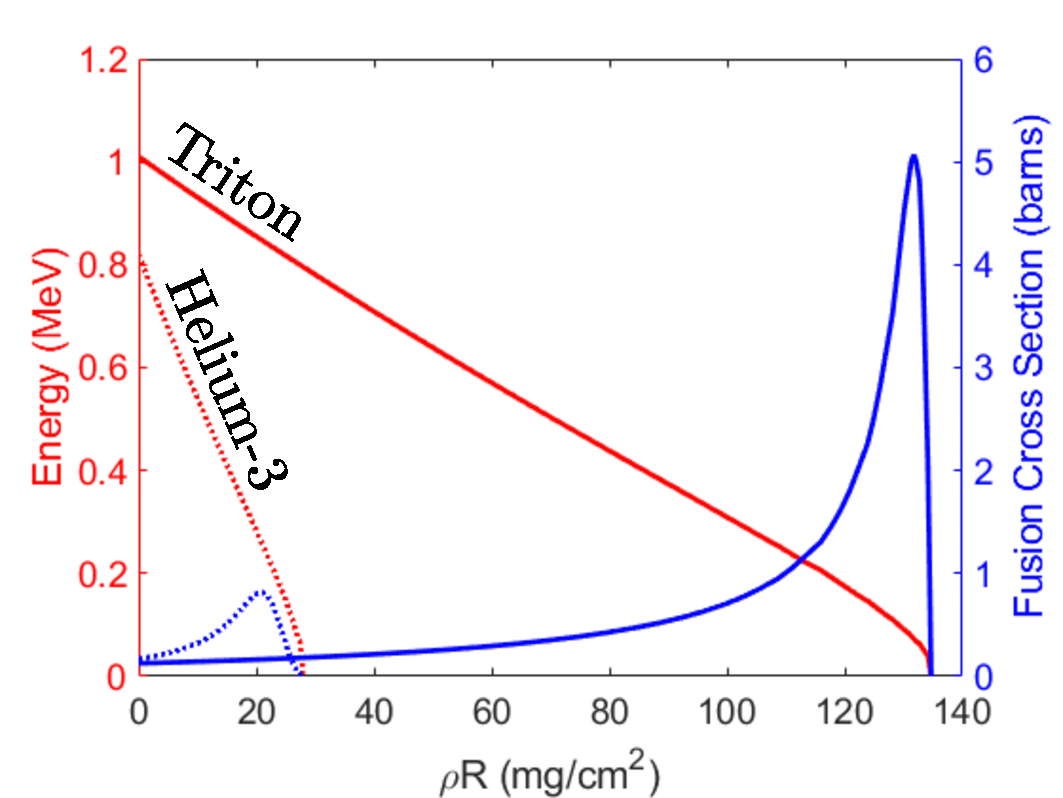
\includegraphics[scale=0.6]{secondaryCrossSection}
		\caption[Secondary fusion cross sections]{Energy and fusion cross sections of primary products as they stream through a deuterium plasma with a temperature of 5 keV and a density of 1 g/cc. The solid lines track the properties of a DD triton and it's probability of undergoing DT fusion and the dashed lines track the properties of a DD helium-3 ion and it's probability of undergoing D$^3$He fusion. Blue curves represent the corresponding cross section and red curves represent the corresponding energy.  }
		\label{secondaryCrossSection}
	\end{figure}
	
	 If the areal density ($\rho R$) of the plasma is sufficiently small, the primary product will stream through the entire plasma in a straight line loosing a minimal amount of energy. In this case, $\sigma_{ij}$ is roughly constant and the path of the secondary particle will be of order $R$, the radius of the plasma. As a result:
	%
	\begin{equation}
		\begin{split}
			\left(\frac{Y_2}{Y_1}\right) 
			& \propto \left<\rho R\right>_j \\
		\end{split}
	\end{equation}
	%
	in this regime. If, alternatively, the areal density is sufficiently high, the secondary particle will not be able to escape the plasma. Instead it will lose all of its energy to Coulomb collisions and become thermalized with the plasma. In this process, $\sigma_{ij}$ will effectively tend to 0 and the yield ratio will asymptote to a fixed value. In other words:
	%
	\begin{equation}
		\begin{split}
			\left(\frac{Y_2}{Y_1}\right) 
			& \sim \text{constant} \\
		\end{split}
	\end{equation}
	%
	in this regime.	Figure \ref{yieldRatioCurves} shows the simulated behavior of the yield ratio as a function of $\rho R$ for a couple secondary nuclear reactions. 
	
	\begin{figure}[h!]
		\centering
		\includegraphics[scale=0.6]{yieldRatio}
		\caption[Secondary Product  Yield Ratios]{Yield ratio of secondary DT reactions (red) and secondary D$^3$He reactions (blue) to their corresponding primary DD reactions. The solid, dashed, and dash-dotted curves correspond to plasma source with temperature equal 8.0, 4.0, and 2.0 keV respectively. For low areal densities, yield ratios are proportional to the areal density and for high areal densities, the yield ratios asymptote to a constant value. The exact saturation value varies with plasma properties such as $T_e$ (illustrated here) and $n_e$. The transition region between the two extremes exist due to the secondary particles having non mono energetic spectras and volumetric birth profiles. These curves were generated using the Monte Carlo model discussed in \todo{where?}. The source plasma was deuterium filled will a uniform 1.0 g/cc density and uniform temperature. Primary product particles were sampled from the corresponding (uniform) DD burn distribution.  }
		\label{yieldRatioCurves}
	\end{figure}

	

	The exact saturation point and value of the yield ratios depends on how much areal density is required to thermalize the primary product in question. This, again, is described by the stopping power of the plasma on said particle. The details of plasma stopping power is itself an entire research topic, but for the purposes of this work it is sufficient to know that it is a strong function of the plasma's electron temperature ($T_e$) and electron density ($n_e$). This means, the saturation points of the yield ratios are themselves a strong function of these parameters. It is important to note, that this dependency only manifests at moderate to high areal densities, that is areal densities of the order of the primary product's maximum range. Below this point, the yield ratio depends only on the areal density of the plasma and is agnostic to other plasma parameters. The behavior is also shown in Figure \ref{yieldRatioCurves}.
	
	These characteristics make the yield ratio of secondary reactions a strong diagnostic tool for integrated plasma conditions. \todo{More}
	
	
\subsection{Secondary Spectra}

	As mentioned, secondary reactions create particles with an enormous range of energies due to the high center of mass energy of the reaction. An example of this is the secondary DT reaction given by equation \ref{secondaryDTn}. More specifically, the different lab energies correspond to the direction the primary product particle was traveling relative to the observer. The exact dependence is shown in equation \ref{Appendix_A_LabFrame_Energy_Theta_Function}. This is also shown plotted in the case of secondary DT neutrons in Figure \ref{secondaryDTnEnergy}.
	
	
	\begin{figure}[h!]
		\centering
		\includegraphics[scale=0.6]{secondaryDTnEnergy}
		\caption[Secondary DT neutron angle-energy relationship]{Relationship between the lab angle $\theta$ and the resulting energy of a secondary DT neutron. The red, blue, and green curves show the case of a 1.0, 0.6, and 0.2 MeV triton resulting in the birth of the neutron. The black dashed line corresponds to the so called \emph{zero-temperature birth energy} of a DT neutron; the case when both parents have exactly 0 energy. While technically $\theta$ in equation \ref{Appendix_A_LabFrame_Energy_Theta_Function} refers to the angle between the triton and the neutron, the angle between the line of sight and the triton is almost exactly equal for any detector any reasonable distance away from the plasma. }
		\label{secondaryDTnEnergy}
	\end{figure}

	As the primary product loses energy in the source plasma, the secondary particle's energy-angle relationship changes. Notably the centroid shifts, and the range of energies becomes narrower. In cases where a significant amount of energy is loss, the resulting spectra will be a convolution of these different relationships. Some example spectra are shown in Figure \ref{secondarySpectra_rhoR}
	
	\begin{figure}[h!]
		\centering
		\includegraphics[scale=0.6]{secondarySpectra_rhoR}
		\caption[Secondary DT neutron spectra for varying areal densities]{Resulting secondary DT neutron spectra from deuterium source plasmas of varying areal densities. Simulations used a uniform density and temperature of 1.0 g/cc and 4 keV respectively. The red, blue, and green curve correspond to areal densities of 20, 60, and 100 mg/cm$^2$. As the areal density increases to and beyond the average range of a 1.01 MeV triton, the spectra gets more narrow and the centroid shifts to lower energies. Like the yield ratio, this behavior has a treshold to it. All spectra below approximately 20 mg/cm$^2$ look identical to one another and all spectra above 100 mg/cm$^2$ look identical as well.}
		\label{secondarySpectra_rhoR}
	\end{figure}
		
	This relationship between lab angle and secondary product energy, means the shape of a measured secondary spectra encode the shape of the source plasma relative to the detector. For low areal density plasmas, every energy uniquely maps to a angle about the detector line of sight. This means that the secondary yield ratio between a given energy ban $E$ to $E+\Delta E$ is a measurement of an azimuthally averaged areal density between angles $\theta(E)$ and $\theta(E+\Delta E)$. For higher areal density plasmas, ranging creates a degeneracy between energy and angle which makes the relationship less clear, but the dependence remains. Examples of spectra from asymmetric plasma sources is shown in Figure \ref{secondaryDTAsym}.
	
	\begin{figure}[h!]
		\centering
		\includegraphics[scale=0.6]{secondaryDTAsym}
		\caption[Secondary DT neutron spectra from asymmetric plasmas]{ Simulated secondary DT neutron spectra from prolate deuterium plasma sources with uniform density and uniform temperature 1.0 g/cc and 4.0 keV respectively. The red (blue) curves are the secondary spectra as measured from the equator (pole). The dashed and solid curves correspond to an average areal density of 10 mg/cm$^2$ and 100 mg/cm$^2$ respectively. The spectral shapes map out the areal density asymmetry relative to their respective lines of sight. Different lines of sight measure different spectra due to their orientations relative to the asymmetries. \todo{list $R(\theta)$}   }
		\label{secondaryDTAsym}
	\end{figure}


